\section{Tooling}\label{sec:tooling}
This chapter describes the tools that we developed while designing an implementing algorithms for scalafmt.
These tools were indispensable in giving us confidence that our algorithms worked as intended.

\subsection{Heatmaps}
Section~\ref{sec:optimizations} introduces several extensions to algorithm~\ref{alg:bfsv1} that were required to get good performance for scalafmt.
In general, the extensions involved eliminating search states.
To identify code patterns that triggered excessive search growth, we used heatmaps.

Heatmaps are a visualization that displays which code regions are most frequently visited in the best-first search.
Figure~\ref{fig:heatmap} shows an example heatmap.
\begin{figure}
  \centering
  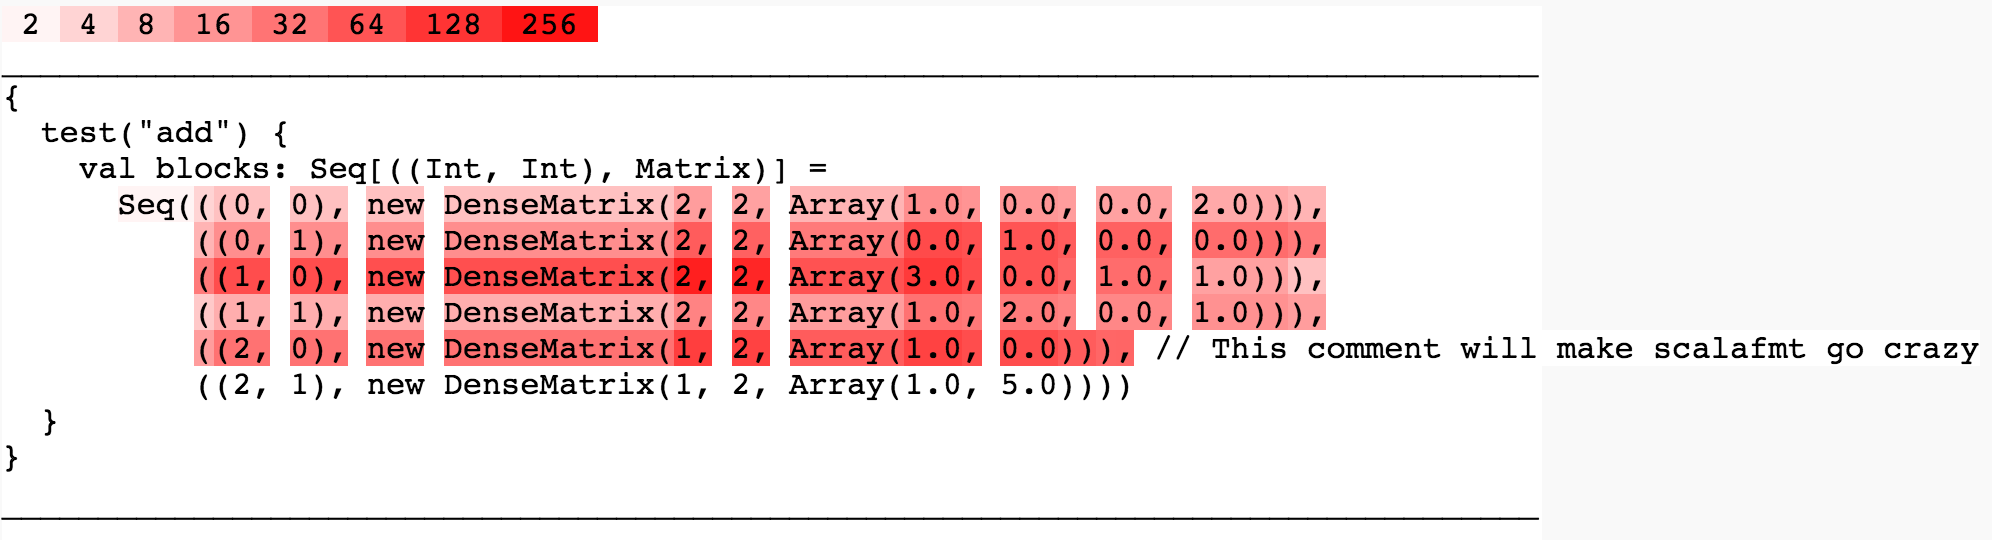
\includegraphics[width=\textwidth]{img/heatmap.png}
  \caption{Example heatmap with 5.121 visisted states}
  \label{fig:heatmap}
\end{figure}
The intensity of the red color indicates how often a particular token was visited.
A token highlighted by the lightest shade of red was visited twice while a token highlighted by the darkest shade of red was visited over 256 times.
This figure demonstrates several of the optimizations discussed in section~\ref{sec:optimizations}.
Firstly, thanks to the \texttt{dequeueOnNewStatements} optimization, the background is plain white up to the second \texttt{Seq}.
The second \texttt{Seq} gets visited twice, once when there's a space after the \texttt{=} and once when there's a newline.
Secondly, due to the OptimalToken optimization, when the search gets into trouble it backtracks to the tuple \texttt{(0, 0)} instead of the \texttt{Seq[((Int, Int), Matrix)]} type signature.
Finally, because of the strategically placed comment at the end that exceeds the column limit, the search space grows out of bounds on the fourth argument triggering the \texttt{escapeInPathologicalCases} best-effort fallback.
Without heatmaps, it would be a much greater challenge to get these insights.
However, these heatmaps gave us limited insights in how our optimizations affected the search space in the best-first search.

We developed an extension to heatmaps that allows us to visually compare the difference in search space between two versions of scalafmt.
Figure~\ref{fig:heatmap2} shows an example of such a report, which we call a \emph{diff heatmap}.
\begin{figure}
  \centering
  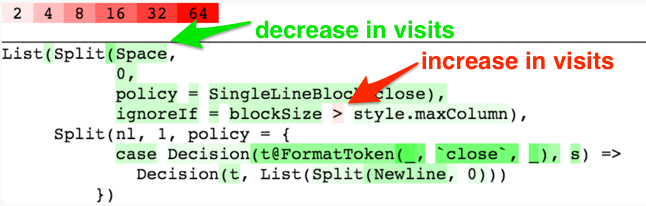
\includegraphics[width=\textwidth]{img/heatmap2-annot.png}
  \caption{Example diff heatmap}
  \label{fig:heatmap2}
\end{figure}
The green background indicates that the new version of scalafmt makes fewer visits to those regions.
Observe that the \texttt{>} operator has a background with a light shade of red.
This means that the operator was visisted more often in the new scalafmt version.
A price well worth paying considering the overall shrink in search space.
To produce diff heatmaps, we first persist statistics from two different heatmaps to a database.
Then, we generate the diff heatmap by fetching the two reports and calculating the difference in visits per token.
If the difference is negative for a particular token --- meaning we visited that token fewer times --- the background is highlighted green, otherwise red.
Diff heatmaps were useful to detect performance regressions when we added or removed optimizations.

\subsection{Property based testing}~\label{sec:testing}
Property based tests played a vital role in the development of scalafmt and gave us confidence that the algorithms from section~\ref{sec:algorithms} behave well against the real world input.
Typically, property based tests run again randomly generated input.
However, generating random source files which might be unrepresentative for human written code.
Instead, we chose to collect a large sample of 1.2 million lines of code from open source Scala projects available online.
The sample was compressed into a 23mb zip file\footnote{See \url{https://github.com/olafurpg/scalafmt/releases/download/v0.1.4/repos.tar.gz}}.
Our test suite would download the sample and test three properties: \emph{can-format}, \emph{AST integrity} and \emph{idempotency}.

\subsubsection{Can-format}
The can-format property simply says that if the Scala compiler's parser is able to parse the source input file, then scalafmt should be able to format the source file.
Although this may seem like a trivial property, it was by far the most effective property at finding bugs in scalafmt.
Most commonly, comments in unexpected placed caused the best-first search to not reach the last token in the input.
An overly strict Policy was usually the culprit of such bugs, which was easy to fix thanks to our tracing techniques described in section~\ref{sec:router}.

\subsubsection{AST integrity}
The AST integrity property says that the abstract syntax tree of the formatted source file should be identical to the abstract syntax tree of the original input.
Recall from section~\ref{sec:scalameta} that scala.meta trees can be serialized into strings.
We leverage this feature to test AST integrity.
Algorithm~\ref{alg:ast} shows the code needed to test AST integrity.
\begin{algorithm}
  \caption{AST integrity property}\label{alg:ast}
  \lstinputlisting[nolol]{code/ast.scala}
\end{algorithm}
This property catched several critical bugs.
For example, in one case, scalafmt inserted a newline after the keyword \texttt{return}, breaking the semantics of the original source code.
Moreover, this property highlighted the danger of enabling \texttt{stripMargin} alignment.
Since the \texttt{stripMargin} modified the contents of regular and interpolated string literals,
the AST of the formatted output changed.
Knowing that scalafmt preserves the AST of the input code gives us great confidence that scalafmt will not introduce bugs in our users code.

\subsubsection{Idempotency}
The idempotency property says that formatting a source file twice should produce the same output as formatting the same file once.
This property is critical for scalafmt to be used as part of any continuous integration setup.
It is not at all obvious that the algorithms in section~\ref{sec:algorithms} fulfill the idempotency property.
Our experience reveals that it is in fact very easy to accidentally introduce non-idempotent formatting rules in the Router.
We did not test for idempotency until the 0.2.3 release, after users reported non-idempotent formatting behavior in scalafmt.
Yet, even after we started testing against idempotency in our comprehensive test-suite, we continued to receive issues with non-idempotent formatting.
This time it appears that the \texttt{escapeInPathologicalCases} strategy from section~\ref{sec:escape} was the culprit.
For the next release, we plan to disable \texttt{escapeInPathologicalCases} by default in favor use its safer alternative.
It turns out that 1.2 million lines of code is not a large enough sample to catch all property bugs.
